\batchmode
\documentstyle[screen,makeidx,ifthen,calc,dingbat,optarg,11pt,epsfig,rotating]{cernman}
\makeatletter
\makeindex

\newenvironment{ICON}[1]{\begin{minipage}{.1\textwidth}
                          \epsfig{file=#1.eps,width=\textwidth}
                          \end{minipage}\hfill
                          \begin{minipage}{.85\textwidth}}                          {\end{minipage}}
\newlength{\Mylen}
\newenvironment{PAWf}[2][.3]
               {\setlength{\Mylen}{.95\textwidth-\textwidth*\real{#1}}               \begin{minipage}{#1\textwidth}
               \epsfig{file=#2.eps,width=\textwidth}
               \end{minipage}\hfill
               \begin{minipage}{\Mylen}}               {\end{minipage}}
\newenvironment{PAWfR}[1]{\begin{minipage}{.3\textwidth}
                          \begin{turn}{-90}                          \mbox{\epsfig{file=#1.eps,height=\textwidth}}
                          \end{turn}
                          \end{minipage}\hfill
                          \begin{minipage}{.65\textwidth}}                          {\end{minipage}}
\newcommand{\MENU}[1]{\begin{center}
                      \mbox{\epsfig{file=#1.eps}}                      \end{center}}
\newcommand{\PAWF}[1]{\begin{center}
                      \mbox{\epsfig{file=#1.eps,width=\textwidth}}                      \end{center}}
\newcommand{\PAWFR}[1]{\begin{turn}{-90}                       \mbox{\epsfig{file=#1.eps,height=\textwidth}}                       \end{turn}}

\sansfont{helvetica}\romanfont{times}

\newcounter{Mycount}
\newcommand{\Denslist}
{\itemsep=0pt\parsep=0pt\partopsep=0pt\topsep=\baselineskip\parskip=0pt}
\newenvironment{EnumZW}{\renewcommand{\labelenumi}
                       {\setcounter{Mycount}{191+\value{enumi}}                       \raisebox{-2pt}[0cm][0cm]
                       {\Large\ding{\the\value{Mycount}}}}                       \enumerate\Denslist}                       {\endlist}
\newenvironment{EnumZB}{\renewcommand{\labelenumi}
                      {\setcounter{Mycount}{201+\value{enumi}}                   \raisebox{-2pt}[0cm][0cm]{\Large\ding{\the\value{Mycount}}}}                        \enumerate\Denslist}                       {\endlist}


\newenvironment{DLsf}[1]                        {\def\DLH{\sf}\begin{DLgen}{#1}}{\end{DLgen}}
\newenvironment{DLsfc}[1]                        {\def\DLH{\sf}\begin{DLgenc}{#1}}{\end{DLgenc}}


\newcommand{\NbDW}[1]{\setcounter{Mycount}{191+#1}\ding{\the\value{Mycount}}}\newcommand{\NbDB}[1]{\setcounter{Mycount}{201+#1}\ding{\the\value{Mycount}}}\newcommand{\Button}[1]{\psboxit{rectcartouche}{\spbox{\footnotesize\sf#1}}}
\newcommand{\Field}[1]{\psboxit{box 0.9 setgray fill}
                      {\spbox{\footnotesize\sf#1}}}

\long\def\psboxit#1#2{\begingroup\setbox0=\hbox{#2}\dimen0=\ht0 \advance\dimen0 by \dp0            \hbox{    \special{ps: gsave currentpoint translate
        0
        \number\dp0 \space 15800 div            \number\wd0 \space 15800 div            \number\ht0 \space -15800 div           #1 grestore}    \copy0}\endgroup}
\long\def\spbox#1{\begingroup\fboxsep=1pt\leavevmode\setbox1\hbox{#1}    \dimen0\fboxrule \advance\dimen0 \fboxsep    \advance\dimen0 \dp1    \hbox{\lower \dimen0\hbox    {\vbox{\hrule height \fboxrule width 0pt          \hbox{\vrule width \fboxrule height 0pt \hskip\fboxsep          \vbox{\vskip\fboxsep \box1\vskip\fboxsep}\hskip                 \fboxsep\vrule width \fboxrule height 0pt}                 \hrule height \fboxrule width 0pt}}}\endgroup}\long\def\PScommands{\special{! TeXDict begin
/box{newpath 2 copy moveto 3 copy pop exch lineto 4 copy pop pop
lineto exch pop exch pop lineto closepath } bind def
/roundedbox{/radius exch store
3 2 roll 2 copy min radius sub /miny exch store max radius add /maxy exch store
2 copy min radius sub /minx exch store max radius add /maxx exch store
newpath
minx radius add miny moveto
maxx miny maxx maxy radius arcto
maxx maxy minx maxy radius arcto
minx maxy minx miny radius arcto
minx miny maxx miny radius arcto 16 {pop} repeat
closepath
}bind def
/rectcartouche{4 copy .9 setgray 3 setlinewidth box fill .5 setgray box stroke
}bind def
/cartouche{5 copy .9 setgray 5 setlinewidth roundedbox fill .95 setgray roundedbox stroke
}bind def
end }}\PScommands
\renewcommand{\CERNLIB}{\textsc{cernlib}\index{CERNLIB}}
\renewcommand{\CMZ}{\textsc{cmz}\index{CMZ}}
\renewcommand{\COMIS}{\textsc{comis}\index{COMIS}}
\renewcommand{\CSPACK}{\textsc{cspack}\index{CSPACK}}
\renewcommand{\FATMEN}{\textsc{fatmen}\index{FATMEN}}
\renewcommand{\GEANT}{\textsc{geant}\index{GEANT}}
\renewcommand{\GKS}{\textsc{gks}\index{GKS}}
\renewcommand{\HBOOK}{\textsc{hbook}\index{HBOOK}}
\renewcommand{\HEPDB}{\textsc{hepdb}\index{HEPDB}}
\renewcommand{\HIGZ}{\textsc{higz}\index{HIGZ}}
\renewcommand{\HPLOT}{\textsc{hplot}\index{HPLOT}}
\renewcommand{\KUIP}{\textsc{kuip}\index{KUIP}}
\renewcommand{\MINUIT}{\textsc{minuit}\index{MINUIT}}
\renewcommand{\PATCHY}{\textsc{patchy}\index{PATCHY}}
\renewcommand{\PAW}{\textsc{paw}\index{PAW}}
\renewcommand{\SIGMA}{\textsc{sigma}\index{SIGMA}}
\renewcommand{\PAWPP}{\textsc{paw++}\index{PAW++}}
\renewcommand{\WWW}{\textsc{www}\index{WWW}}
\renewcommand{\VAXTAP}{\textsc{vaxtap}\index{VAXTAP}}
\renewcommand{\ZEBRA}{\textsc{zebra}\index{ZEBRA}}


\newcommand{\RZ}{{\sf RZ}\index{RZ}}
\newcommand{\PHIGS}{{\sf PHIGS}\index{PHIGS}}
\newcommand{\GPHIGS}{{\sf GPHIGS}\index{GPHIGS}}
\newcommand{\XPAW}{{\sf PAW}\index{PAW (Physics Analysis Workstation)}}
\newcommand{\PS}{{\sf Post\-Script}\index{PostScript}}
\newcommand{\EPS}{{\sf En\-cap\-su\-la\-ted Post\-Script}\index{PostScript!Encapsulated}}
\newcommand{\FALCO}{{\sf FALCO}\index{FALCO}}
\newcommand{\MSDOS}{{\sf MSDOS}\index{MSDOS}}
\newcommand{\MAC}{{\sf MacIntosh}\index{MacIntosh}}
\newcommand{\GDDM}{{\sf GDDM}\index{GDDM}}
\newcommand{\XW}{{\sf X Window System}\index{X Window System}}
\newcommand{\Xxi}{{\sf X11}\index{X11}}
\newcommand{\GL}{{\sf GL}\index{GL}}
\newcommand{\GPR}{{\sf GPR}\index{GPR}}
\newcommand{\GMR}{{\sf GMR}\index{GMR}}
\newcommand{\MOTIF}{{\sf Motif}\index{Motif}}
\newcommand{\XLIB}{{\sf Xlib}\index{Xlib}}

\newcommand{\NDC}{normalized device coordinates\index{coordinates!normalized device}}
\newcommand{\DC}{device coordinates\index{coordinates!device}}
\newcommand{\WC}{world coordinates\index{coordinates!world}}

\newcommand{\ndc}{{\sf NDC}\index{coordinates!normalized device}}
\newcommand{\dc}{{\sf DC}\index{coordinates!device}}
\newcommand{\wc}{{\sf WC}\index{coordinates!world}}

\newcommand{\FORTRAN}{{\sf Fortran}\index{Fortran}}
\newcommand{\CHARACTER}{{\tt CHARACTER}}

\newcommand{\UGP}{underlying graphics package\index{underlying graphics package}}
\newcommand{\UGPs}{underlying graphics packages\index{underlying graphics package}}

\newcommand{\TELNETG}{{\sf Telnetg}\index{Telnetg}}

\newcommand{\HW}{{\tt higz\_windows.dat}\index{higzwindows.dat}}

\newcommand{\nt}{{\sf NT}\index{normalization transformation}}
\newcommand{\wt}{{\sf WT}\index{workstation transformation}}

\newcommand{\NT}{normalization transformation\index{normalization transformation}}
\newcommand{\NTs}{normalization transformations\index{normalization transformation}}
\newcommand{\WT}{workstation transformation\index{workstation transformation}}
\newcommand{\WTs}{workstation transformations\index{workstation transformation}}
\newcommand{\ASCII}{{\tt ASCII}\index{ASCII}}

\newcommand{\UNIX}{{\sf UNIX}\index{UNIX}}
\newcommand{\VMS}{{\sf VAX/VMS}\index{VAX/VMS}}

\newcommand{\MB}{{\bf Main Browser}\index{Main Browser}}
\newcommand{\EW}{{\bf Executive Window}\index{Executive Window}}
\newcommand{\TP}{{\bf Transcript Pad}\index{Transcript Pad}}
\newcommand{\IP}{{\bf Input Pad}\index{Input Pad}}
\newcommand{\NV}{{\bf Ntuple Viewer}\index{Ntuple Viewer}}
\newcommand{\HSP}{{\bf Histogram Style Panel}\index{Histogram Style Panel}}
\newcommand{\PL}{{\bf PAW++ Locate}\index{PAW++ Locate}}
\newcommand{\GW}{{\bf Graphics Window}\index{Graphics Window}}
\newcommand{\CE}{{\bf Cut Editor}\index{Cut Editor}}



\def\psboxit#1#2{\begingroup\setbox0=\hbox{#2}\dimen0=\ht0 \advance\dimen0 by \dp0            \hbox{    \special{ps: gsave currentpoint translate
        0
        \number\dp0 \space 15800 div            \number\wd0 \space 15800 div            \number\ht0 \space -15800 div           #1 grestore}    \copy0}\endgroup}\def\spbox#1{\begingroup\fboxsep=1pt\leavevmode\setbox1\hbox{#1}    \dimen0\fboxrule \advance\dimen0 \fboxsep    \advance\dimen0 \dp1    \hbox{\lower \dimen0\hbox    {\vbox{\hrule height \fboxrule width 0pt          \hbox{\vrule width \fboxrule height 0pt \hskip\fboxsep          \vbox{\vskip\fboxsep \box1\vskip\fboxsep}\hskip                 \fboxsep\vrule width \fboxrule height 0pt}                 \hrule height \fboxrule width 0pt}}}\endgroup}\def\PScommands{\special{! TeXDict begin
/box{newpath 2 copy moveto 3 copy pop exch lineto 4 copy pop pop
lineto exch pop exch pop lineto closepath } bind def
/roundedbox{/radius exch store
3 2 roll 2 copy min radius sub /miny exch store max radius add /maxy exch store
2 copy min radius sub /minx exch store max radius add /maxx exch store
newpath
minx radius add miny moveto
maxx miny maxx maxy radius arcto
maxx maxy minx maxy radius arcto
minx maxy minx miny radius arcto
minx miny maxx miny radius arcto 16 {pop} repeat
closepath
}bind def
/rectcartouche{4 copy .9 setgray 3 setlinewidth box fill .5 setgray box stroke
}bind def
/cartouche{5 copy .9 setgray 5 setlinewidth roundedbox fill .95 setgray roundedbox stroke
}bind def
end }}\renewcommand{\CERNLIB}{\textsc{cernlib}\index{CERNLIB}}\renewcommand{\CMZ}{\textsc{cmz}\index{CMZ}}\renewcommand{\COMIS}{\textsc{comis}\index{COMIS}}\renewcommand{\CSPACK}{\textsc{cspack}\index{CSPACK}}\renewcommand{\FATMEN}{\textsc{fatmen}\index{FATMEN}}\renewcommand{\GEANT}{\textsc{geant}\index{GEANT}}\renewcommand{\GKS}{\textsc{gks}\index{GKS}}\renewcommand{\HBOOK}{\textsc{hbook}\index{HBOOK}}\renewcommand{\HEPDB}{\textsc{hepdb}\index{HEPDB}}\renewcommand{\HIGZ}{\textsc{higz}\index{HIGZ}}\renewcommand{\HPLOT}{\textsc{hplot}\index{HPLOT}}\renewcommand{\KUIP}{\textsc{kuip}\index{KUIP}}\renewcommand{\MINUIT}{\textsc{minuit}\index{MINUIT}}\renewcommand{\PATCHY}{\textsc{patchy}\index{PATCHY}}\renewcommand{\PAW}{\textsc{paw}\index{PAW}}\renewcommand{\SIGMA}{\textsc{sigma}\index{SIGMA}}\renewcommand{\PAWPP}{\textsc{paw++}\index{PAW++}}\renewcommand{\WWW}{\textsc{www}\index{WWW}}\renewcommand{\VAXTAP}{\textsc{vaxtap}\index{VAXTAP}}\renewcommand{\ZEBRA}{\textsc{zebra}\index{ZEBRA}}\def\Ptitle#1{\special{ps: /Printstring (#1) def}
\epsfbox{/user/goossens/cnasall/cnastit.eps}}\renewcommand{\arraystretch}{.9}
\makeatother
\newenvironment{tex2html_wrap}{}{}
\setlength{\textheight}{100in}\begin{document}
\pagestyle{empty}
\newpage

{\samepage \clearpage \special{! TeXDict begin
/box{newpath 2 copy moveto 3 copy pop exch lineto 4 copy pop pop
lineto exch pop exch pop lineto closepath } bind def
/roundedbox{/radius exch store
3 2 roll 2 copy min radius sub /miny exch store max radius add /maxy exch store
2 copy min radius sub /minx exch store max radius add /maxx exch store
newpath
minx radius add miny moveto
maxx miny maxx maxy radius arcto
maxx maxy minx maxy radius arcto
minx maxy minx miny radius arcto
minx miny maxx miny radius arcto 16 {pop} repeat
closepath
}bind def
/rectcartouche{4 copy .9 setgray 3 setlinewidth box fill .5 setgray box stroke
}bind def
/cartouche{5 copy .9 setgray 5 setlinewidth roundedbox fill .95 setgray roundedbox stroke
}bind def
end }\ 
}


\newpage

{\samepage \clearpage \framebox
}


\newpage

{\samepage \clearpage \begin{tabular}{l@{\qquad}l@{\quad}>{\tt}l}
{\em Contact Person\/}:        & Ren\'e Brun /CN     & (BRUN\atsign CERNVM.CERN.CH)    \\  
{\em Technical Realization\/}: & Michel Goossens /CN & (GOOSSENS\atsign CERNVM.CERN.CH)\\  [1cm]
{\em First edition - September 1993}
\end{tabular}
}


\newpage

{\samepage \clearpage \begin{tabular}{l}
CERN Program Library Office              \\  
CERN-CN Division                         \\  
CH-1211 Geneva 23                        \\  
Switzerland                              \\  
Tel.      +41 22 767 4951                \\  
Fax.      +41 22 767 7155                \\  
Bitnet:   CERNLIB@CERNVM                 \\  
DECnet:   VXCERN::CERNLIB (node 22.190)  \\  
Internet: CERNLIB@CERNVM.CERN.CH
\end{tabular}
}


\newpage

{\samepage \clearpage \begin{UL}\item PAW, Physics Analysis Workstation, The Complete Reference~\cite{bib-PAW}
\item COMIS, Compilation and Interpretation System~\cite{bib-COMIS}
\item HBOOK User Guide --- Version 4~\cite{bib-HBOOK}
\item HIGZ --- High level Interface to Graphics and ZEBRA~\cite{bib-HIGZ}
\item HPLOT User Guide --- Version 5~\cite{bib-HPLOT}
\item KUIP --- Kit for a User Interface Package~\cite{bib-KUIP}
\item MINUIT --- Function Minimization and Error Analysis~\cite{bib-MINUIT}
\item ZEBRA --- Data Structure Management System~\cite{bib-ZEBRA}
\end{UL}
}


\newpage

{\samepage \clearpage \LaTeX
}


\newpage

{\samepage \clearpage \begin{tabular}{@{\hspace{5mm}}>{\tt}l}
\underline{ftp asis01.cern.ch}\\  
Trying 128.141.201.136...\\  
Connected to asis01.cern.ch.\\  
220 asis01 FTP server (Version 6.10 Mon Apr 13 15:59:17 MET DST 1992) ready.\\  
Name (asis01:username): \underline{anonymous}\\  
331 Guest login ok, send e-mail address as password.\\  
Password: \underline{your\_{}mailaddress}\\  
ftp> \underline{cd cernlib/do\c cps.dir}\\  
ftp> \underline{get paw++.ps}\\  
ftp> \underline{quit}\\  
\end{tabular}
}


\stepcounter{chapter}
\stepcounter{section}
\newpage

{\samepage \clearpage \begin{UL}\item The upper left corner is the \PAWPP{} {\bf Executive Window}\index{Executive Window}, with its {\bf Input Pad}\index{Input Pad}{}
      at the bottom and the {\bf Transcript Pad}\index{Transcript Pad}{} at the top.
\item The \PAWPP{} Browser, where the various entities (pictures, 1-D and
      2-D histograms and Ntuples) are all defined with their own symbol,
      is shown bottom left.  A ``pop-up'' menu has been activated for the 
      chosen 1-D histogram. Several actions like \Lit{Plot}, \Lit{Smooth},
      \Lit{Fit} etc... can be performed via this menu.
\item The {\bf Graphics Window}\index{Graphics Window}{} is seen top right. 
      A 1-D view of the data points and two 2-D views (a Surface-plot and a 
      colored contour plot) are shown.
      On the 1-D view, two 1-D histograms are 
      superimposed. The results of a ``smoothing'' type of fit to the data 
      points is also drawn. Information about the data and the fit can be found
      in the inserted window.
\item The {\bf Histogram Style Panel}\index{Histogram Style Panel}{} at the lower right allows graphics
      attributes of the histogram to be controlled.
\end{UL}
}


\newpage

{\samepage \clearpage \begin{UL}\item The upper left corner shows the {\bf Ntuple Viewer}\index{Ntuple Viewer}.
      The left window shows the name of the various variables, characterizing
      the selected Ntuple. Other windows and press-buttons specify which
      combinations of the various variables and which events
      have to be treated (plotted, scanned, \ldots).
\item The lower left contains the \PAWPP{} Browser, with this time an Ntuple
      selected. A double on a Ntuple icon
      open automatically the {\bf Ntuple Viewer}\index{Ntuple Viewer}{} on the active Ntuple.
\item The {\bf Graphics Window}\index{Graphics Window}{} is seen top right and shows a 3-D view
      of the combination of three variables, whose cuts are
      specified with the {\bf Cut Editor}\index{Cut Editor}{} (see below).
\item Direct graphics interactions with Ntuple data are possible. Just
      by clicking on a point in the  {\bf Graphics Window}\index{Graphics Window}, the event description is displayed
      in the {\bf PAW++ Locate}\index{PAW++ Locate}{} window.
\item The {\bf Cut Editor}\index{Cut Editor}{} panel, shown at the lower right, allows
      various combinations of cuts to be specified and applied.
\end{UL}
}


\stepcounter{section}
\newpage

{\samepage \clearpage \special{ps: gsave currentpoint translate
        0
        \number\dp0 \space 15800 div            \number\wd0 \space 15800 div            \number\ht0 \space -15800 div           rectcartouche grestore}\ 
}


\stepcounter{subsection}
\newpage

{\samepage \clearpage \begin{turn}{-90}                       \mbox{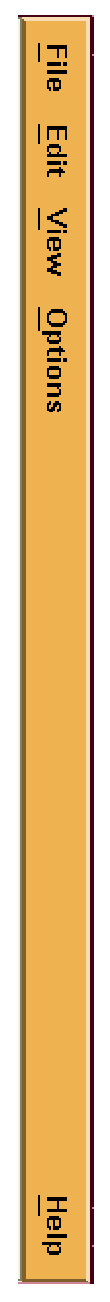
\epsfig{file=menu1.eps,height=\textwidth}}                       \end{turn}
}


\stepcounter{subsubsection}
\stepcounter{subsubsection}
\stepcounter{subsubsection}
\stepcounter{subsubsection}
\stepcounter{subsubsection}
\stepcounter{section}
\stepcounter{subsection}
\stepcounter{subsubsection}
\stepcounter{subsubsection}
\stepcounter{subsubsection}
\stepcounter{subsubsection}
\stepcounter{subsubsection}
\stepcounter{subsubsection}
\stepcounter{subsubsection}
\stepcounter{subsubsection}
\stepcounter{subsubsection}
\stepcounter{subsubsection}
\stepcounter{subsubsection}
\stepcounter{subsubsection}
\stepcounter{subsubsection}
\stepcounter{subsubsection}
\stepcounter{subsubsection}
\stepcounter{subsubsection}
\stepcounter{subsubsection}
\stepcounter{subsubsection}
\stepcounter{subsubsection}
\stepcounter{subsubsection}
\stepcounter{subsubsection}
\stepcounter{subsubsection}
\stepcounter{subsection}
\stepcounter{subsubsection}
\stepcounter{subsubsection}
\stepcounter{subsubsection}
\stepcounter{subsubsection}
\stepcounter{subsubsection}
\stepcounter{subsection}
\stepcounter{subsubsection}
\stepcounter{subsubsection}
\stepcounter{subsection}
\stepcounter{subsubsection}
\stepcounter{subsubsection}
\stepcounter{subsubsection}
\stepcounter{subsubsection}
\stepcounter{subsubsection}
\stepcounter{subsubsection}
\stepcounter{subsubsection}
\stepcounter{subsubsection}
\stepcounter{section}
\stepcounter{subsection}
\stepcounter{subsection}
\stepcounter{subsection}
\stepcounter{subsection}
\stepcounter{subsection}
\stepcounter{subsection}
\stepcounter{subsection}
\stepcounter{subsection}
\stepcounter{subsection}
\stepcounter{section}
\stepcounter{subsection}
\stepcounter{subsubsection}
\stepcounter{subsubsection}
\newpage

{\samepage \clearpage \special{ps: gsave currentpoint translate
        0
        \number\dp0 \space 15800 div            \number\wd0 \space 15800 div            \number\ht0 \space -15800 div           rectcartouche grestore}\ 
}


\stepcounter{subsection}
\stepcounter{subsubsection}
\stepcounter{subsubsection}
\stepcounter{subsubsection}
\stepcounter{subsubsection}
\stepcounter{subsection}
\stepcounter{subsection}
\newpage

{\samepage \clearpage \begin{turn}{-90}                       \mbox{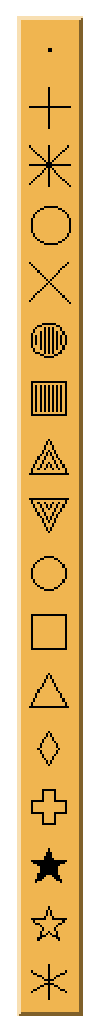
\epsfig{file=marker.eps,height=\textwidth}}                       \end{turn}
}


\stepcounter{subsubsection}
\stepcounter{subsection}
\stepcounter{subsubsection}
\stepcounter{subsubsection}
\stepcounter{subsection}
\stepcounter{subsection}
\stepcounter{subsection}
\stepcounter{subsection}
\stepcounter{subsection}
\stepcounter{subsubsection}
\stepcounter{subsubsection}
\stepcounter{subsection}
\stepcounter{subsection}
\stepcounter{subsection}
\stepcounter{section}
\newpage

{\samepage \clearpage \special{ps: gsave currentpoint translate
        0
        \number\dp0 \space 15800 div            \number\wd0 \space 15800 div            \number\ht0 \space -15800 div           box 0.9 setgray fill grestore}\ 
}


\newpage

{\samepage \clearpage \special{ps: gsave currentpoint translate
        0
        \number\dp0 \space 15800 div            \number\wd0 \space 15800 div            \number\ht0 \space -15800 div           box 0.9 setgray fill grestore}\ 
}


\newpage

{\samepage \clearpage \special{ps: gsave currentpoint translate
        0
        \number\dp0 \space 15800 div            \number\wd0 \space 15800 div            \number\ht0 \space -15800 div           box 0.9 setgray fill grestore}\ 
}


\newpage

{\samepage \clearpage \special{ps: gsave currentpoint translate
        0
        \number\dp0 \space 15800 div            \number\wd0 \space 15800 div            \number\ht0 \space -15800 div           rectcartouche grestore}\ 
}


\newpage

{\samepage \clearpage \special{ps: gsave currentpoint translate
        0
        \number\dp0 \space 15800 div            \number\wd0 \space 15800 div            \number\ht0 \space -15800 div           rectcartouche grestore}\ 
}


\newpage

{\samepage \clearpage \special{ps: gsave currentpoint translate
        0
        \number\dp0 \space 15800 div            \number\wd0 \space 15800 div            \number\ht0 \space -15800 div           box 0.9 setgray fill grestore}\ 
}


\newpage

{\samepage \clearpage \special{ps: gsave currentpoint translate
        0
        \number\dp0 \space 15800 div            \number\wd0 \space 15800 div            \number\ht0 \space -15800 div           box 0.9 setgray fill grestore}\ 
}


\newpage

{\samepage \clearpage \special{ps: gsave currentpoint translate
        0
        \number\dp0 \space 15800 div            \number\wd0 \space 15800 div            \number\ht0 \space -15800 div           box 0.9 setgray fill grestore}\ 
}


\newpage

{\samepage \clearpage \special{ps: gsave currentpoint translate
        0
        \number\dp0 \space 15800 div            \number\wd0 \space 15800 div            \number\ht0 \space -15800 div           rectcartouche grestore}\ 
}


\newpage

{\samepage \clearpage \special{ps: gsave currentpoint translate
        0
        \number\dp0 \space 15800 div            \number\wd0 \space 15800 div            \number\ht0 \space -15800 div           rectcartouche grestore}\ 
}


\newpage

{\samepage \clearpage \special{ps: gsave currentpoint translate
        0
        \number\dp0 \space 15800 div            \number\wd0 \space 15800 div            \number\ht0 \space -15800 div           box 0.9 setgray fill grestore}\ 
}


\newpage

{\samepage \clearpage \special{ps: gsave currentpoint translate
        0
        \number\dp0 \space 15800 div            \number\wd0 \space 15800 div            \number\ht0 \space -15800 div           rectcartouche grestore}\ 
}


\newpage

{\samepage \clearpage \special{ps: gsave currentpoint translate
        0
        \number\dp0 \space 15800 div            \number\wd0 \space 15800 div            \number\ht0 \space -15800 div           rectcartouche grestore}\ 
}


\newpage

{\samepage \clearpage \special{ps: gsave currentpoint translate
        0
        \number\dp0 \space 15800 div            \number\wd0 \space 15800 div            \number\ht0 \space -15800 div           rectcartouche grestore}\ 
}


\newpage

{\samepage \clearpage \special{ps: gsave currentpoint translate
        0
        \number\dp0 \space 15800 div            \number\wd0 \space 15800 div            \number\ht0 \space -15800 div           rectcartouche grestore}\ 
}


\stepcounter{section}
\stepcounter{subsection}
\stepcounter{subsubsection}
\stepcounter{subsubsection}
\stepcounter{subsubsection}
\stepcounter{subsection}
\stepcounter{section}
\appendix
\stepcounter{chapter}
\stepcounter{section}
\stepcounter{section}
\stepcounter{chapter}
\stepcounter{chapter}
\stepcounter{section}
\stepcounter{section}
\stepcounter{subsection}
\stepcounter{subsection}
\stepcounter{subsection}
\stepcounter{section}
\stepcounter{section}
\stepcounter{chapter}

\end{document}